\documentclass[a4paper,11pt]{article}

\usepackage[frenchb]{babel}
\usepackage[utf8]{inputenc}
%\usepackage{verbatim}
\usepackage{graphicx}
\usepackage{listings}
\usepackage{color}

\definecolor{dkgreen}{rgb}{0,0.6,0}
\definecolor{gray}{rgb}{0.5,0.5,0.5}
\definecolor{mauve}{rgb}{0.58,0,0.82}

\lstset{frame=tb,
  language=Java,
  aboveskip=3mm,
  belowskip=3mm,
  showstringspaces=false,
  columns=flexible,
  basicstyle={\small\ttfamily},
  numbers=none,
  numberstyle=\tiny\color{gray},
  keywordstyle=\color{blue},
  commentstyle=\color{dkgreen},
  stringstyle=\color{mauve},
  breaklines=true,
  breakatwhitespace=true,
  tabsize=3
}

\begin{document}
\title{Compte Rendu du TD numéro 7 de l'équipe Eirb'Reteau}
\date{Pour le 18 novembre 2014}
\maketitle

\begin{center}
  Coordinateur : Aurélien Nizet \\
  Tandem 1 : Pierre Gaulon, Victor Dury \\
  Tandem 2 : Lionel Adotevi, Reda Boudjeltia  \\
\end{center}
\maketitle
\section{Introduction}
Faisons un point sur l'avancement de notre code. Jusqu'à maintenant, nous avons deux branches totalement opérationnelles : publique et factory, avec des tests unitaires pour chaque méthode. Cependant, ces tests ne permettent pas de gérer des cas autorisés par le code mais ne représentant pas d'état cohérent, comme par exemple une instanciation d'un bus avec un nombre de places assises négatif. C'est pour gérer cela que nous avons mis au point lors d'une première partie de ce TD7 un système de gestion d'exceptions. Et dans une deuxième partie nous avons modifié la manière de stocker les passagers d'un autobus, au lieu d'utiliser un tableau nous utilisons dorénavant une Collection qui s'avère être un choix plus judicieux.

\section{Gestion d’erreurs et instanciation}
En premier lieu, on peut tester le comportement de notre code lors d'une instance avec des paramètres non valides. Prenons par exemple cette instanciation d'une JaugeNaturel :
\begin{lstlisting}
public void testExceptionCasLimites() {
JaugeNaturel inverse = new JaugeNaturel(-42, -10); 
}
\end{lstlisting}
Dans cet exemple, la JaugeNaturel est bleu et rouge mais pas verte, c'est un état qui n'est pas cohérent. Pour repérer ce type d'erreur, nous allons alors lever des exceptions. \\

\subsection{Lever une exception}
 Nous allons donc lever des exceptions à l'instanciation, pour cela il nous suffit de rajouter une condition sur les paramètres dans les constructeurs à changer et lever l'exception lorsque ces paramètres ne sont pas valides.\\

\subsection{Capturer une exception}
Pour exploiter nos exceptions, il nous faut les capturer et ainsi utiliser les deux blocs $try$ et $catch$. Dans le cas présent, on utilise une variable $inverse$ qu'on déclare et initialise à NULL avant les blocs try et catch pour pouvoir être utilisé par ces derniers. \\
Dans la partie catch, la variable $inverse$ aura la même valeur que lors de son initialisation, car dans le try on va essayer de l'instancier avec des paramètres négatifs et donc non valides, et comme nous avons modifié le constructeur auparavant, on sait que l'instanciation ne va pas aboutir. \\
Si on cherche par exemple à utiliser la variable $inverse$ dans le bloc catch, le compilateur va nous donner un message d'erreur à la compilation car on n'exécute pas forcément le bloc try, et de ce fait on n'instancie pas forcément la variable $inverse$. \\

\section{Paquetage tec}
Nous allons maintenant utiliser les exceptions dans le reste de notre code, et principalement des exceptions contrôlées, celles-ci sont particulièrement utiles car si elle ne sont pas capturées, le compilateur va nous envoyer un message d'erreur, ce qui nous force à gérer toutes les exceptions et donc d'avoir un code plus fiable !\\

\subsection{Exceptions contrôlées}
En particulier nous créons la classe TecInvalidException pour nos exceptions contrôlées, cette dernière hérite de la classe java.lang.Exception, classe mère de toutes les classes d'exceptions contrôlées. \\
Nous utilisons deux constructeurs de TecInvalidException, l'un pour créer une exception sans message associé :
\begin{lstlisting}
 TecInvalidException() {
	super(); 
    }
\end{lstlisting}
L'autre pour créer une exception avec la cause qui est une autre exception que l'on récupère avec un bloc catch (uniquement utilisé dans allerArretSuivant) :
\begin{lstlisting}
 TecInvalidException(String s, Throwable cause) {
	super(s, cause); 
    }
\end{lstlisting}

\subsection{Utilisation des exceptions contrôlées et non-contrôlées}
Il s'agit ici d'implémenter des exceptions contrôlées dans les méthodes $monterDans$ et $allerArretSuivant$. Pour les blocs try et catch de choixChangerPlace, on écrit dans le prototype des méthodes demanderChangerEnAssis et demanderChangerenDebout de Autobus.java "throws IllegalStateException". Ce rajout au prototype se fera par toutes les méthodes qui appellent directement, ou indirectement ces deux méthodes d'Autobus.java. \\
Dans la méthode $allerArretSuivant$, on va "throw new IllegalStateException()" si un passager demande une place assise alors qu'il est déjà assis, ou s'il demande une place debout s'il est déjà debout, et on fait remonter les exceptions jusqu'à cette méthode. Pour la méthode $monterDans$, une exception est levée si le paramètre de cette méthode n'est pas une instance de Bus, pour contrôler la validité du cast dans cette méthode.
Nous avons rajouté des exceptions contrôlées pour les cas de demande incohérentes comme par exemple lorsqu'un passager demande à sortir et qu'il est déjà dehors; et des exceptions non contrôlées pour les cas ou on instancie un bus avec des places négatives, ou on instancie un PassagerAbstrait avec une destination négative. \\

\section{Remplacement d'un tableau par une collection}
Nous abordons ici la deuxième partie du TD qui consiste à remplacer la méthode de stockage avec un tableau par une Collection.

\subsection{Java Collection Framework}

Pour ce changement de méthode de stockage, nous utilisons la Java Collection Framework. Les interfaces Collection, List, Set et Map du conteneur représentent le contrat que doivent respecter les différentes implémentations listées en dessous. Ces interfaces regroupent les méthodes que l'utilisateur pourra appeler pour utiliser ce type de type de données.\\

L'interface Collection permet de répondre aux problèmes que les tableaux peuvent présenter lors du stockage de données. Elle représente des TAD tels que les listes set ou tables de Hashage.\\

L'interface List représente tous les types de listes (LinkedList et ArrayList). Ils permettent de stocker des données sans conditions particulieres.\\

L'interface Set représente tous les types d'ensembles (HashSet, TreeSet, LinkedHashSet). Ils permettent de stocker des objets de façon à les avoir qu'une unique fois.\\

L'interface Map représente les objets qui gèrent les collections sous la forme clé/valeur (HasMap, TreeMap, LinkedHashMap). Ils fonctionnent avec un couple {clé, valeur} pour ranger et retrouver les objets qu'elles contiennent.\\

Voir le diagramme de classe ci-dessous pour l'agencement de ces différentes interfaces : \\
\begin{figure}[!h]
  \begin{center}
    \caption{Diagramme de classes}
    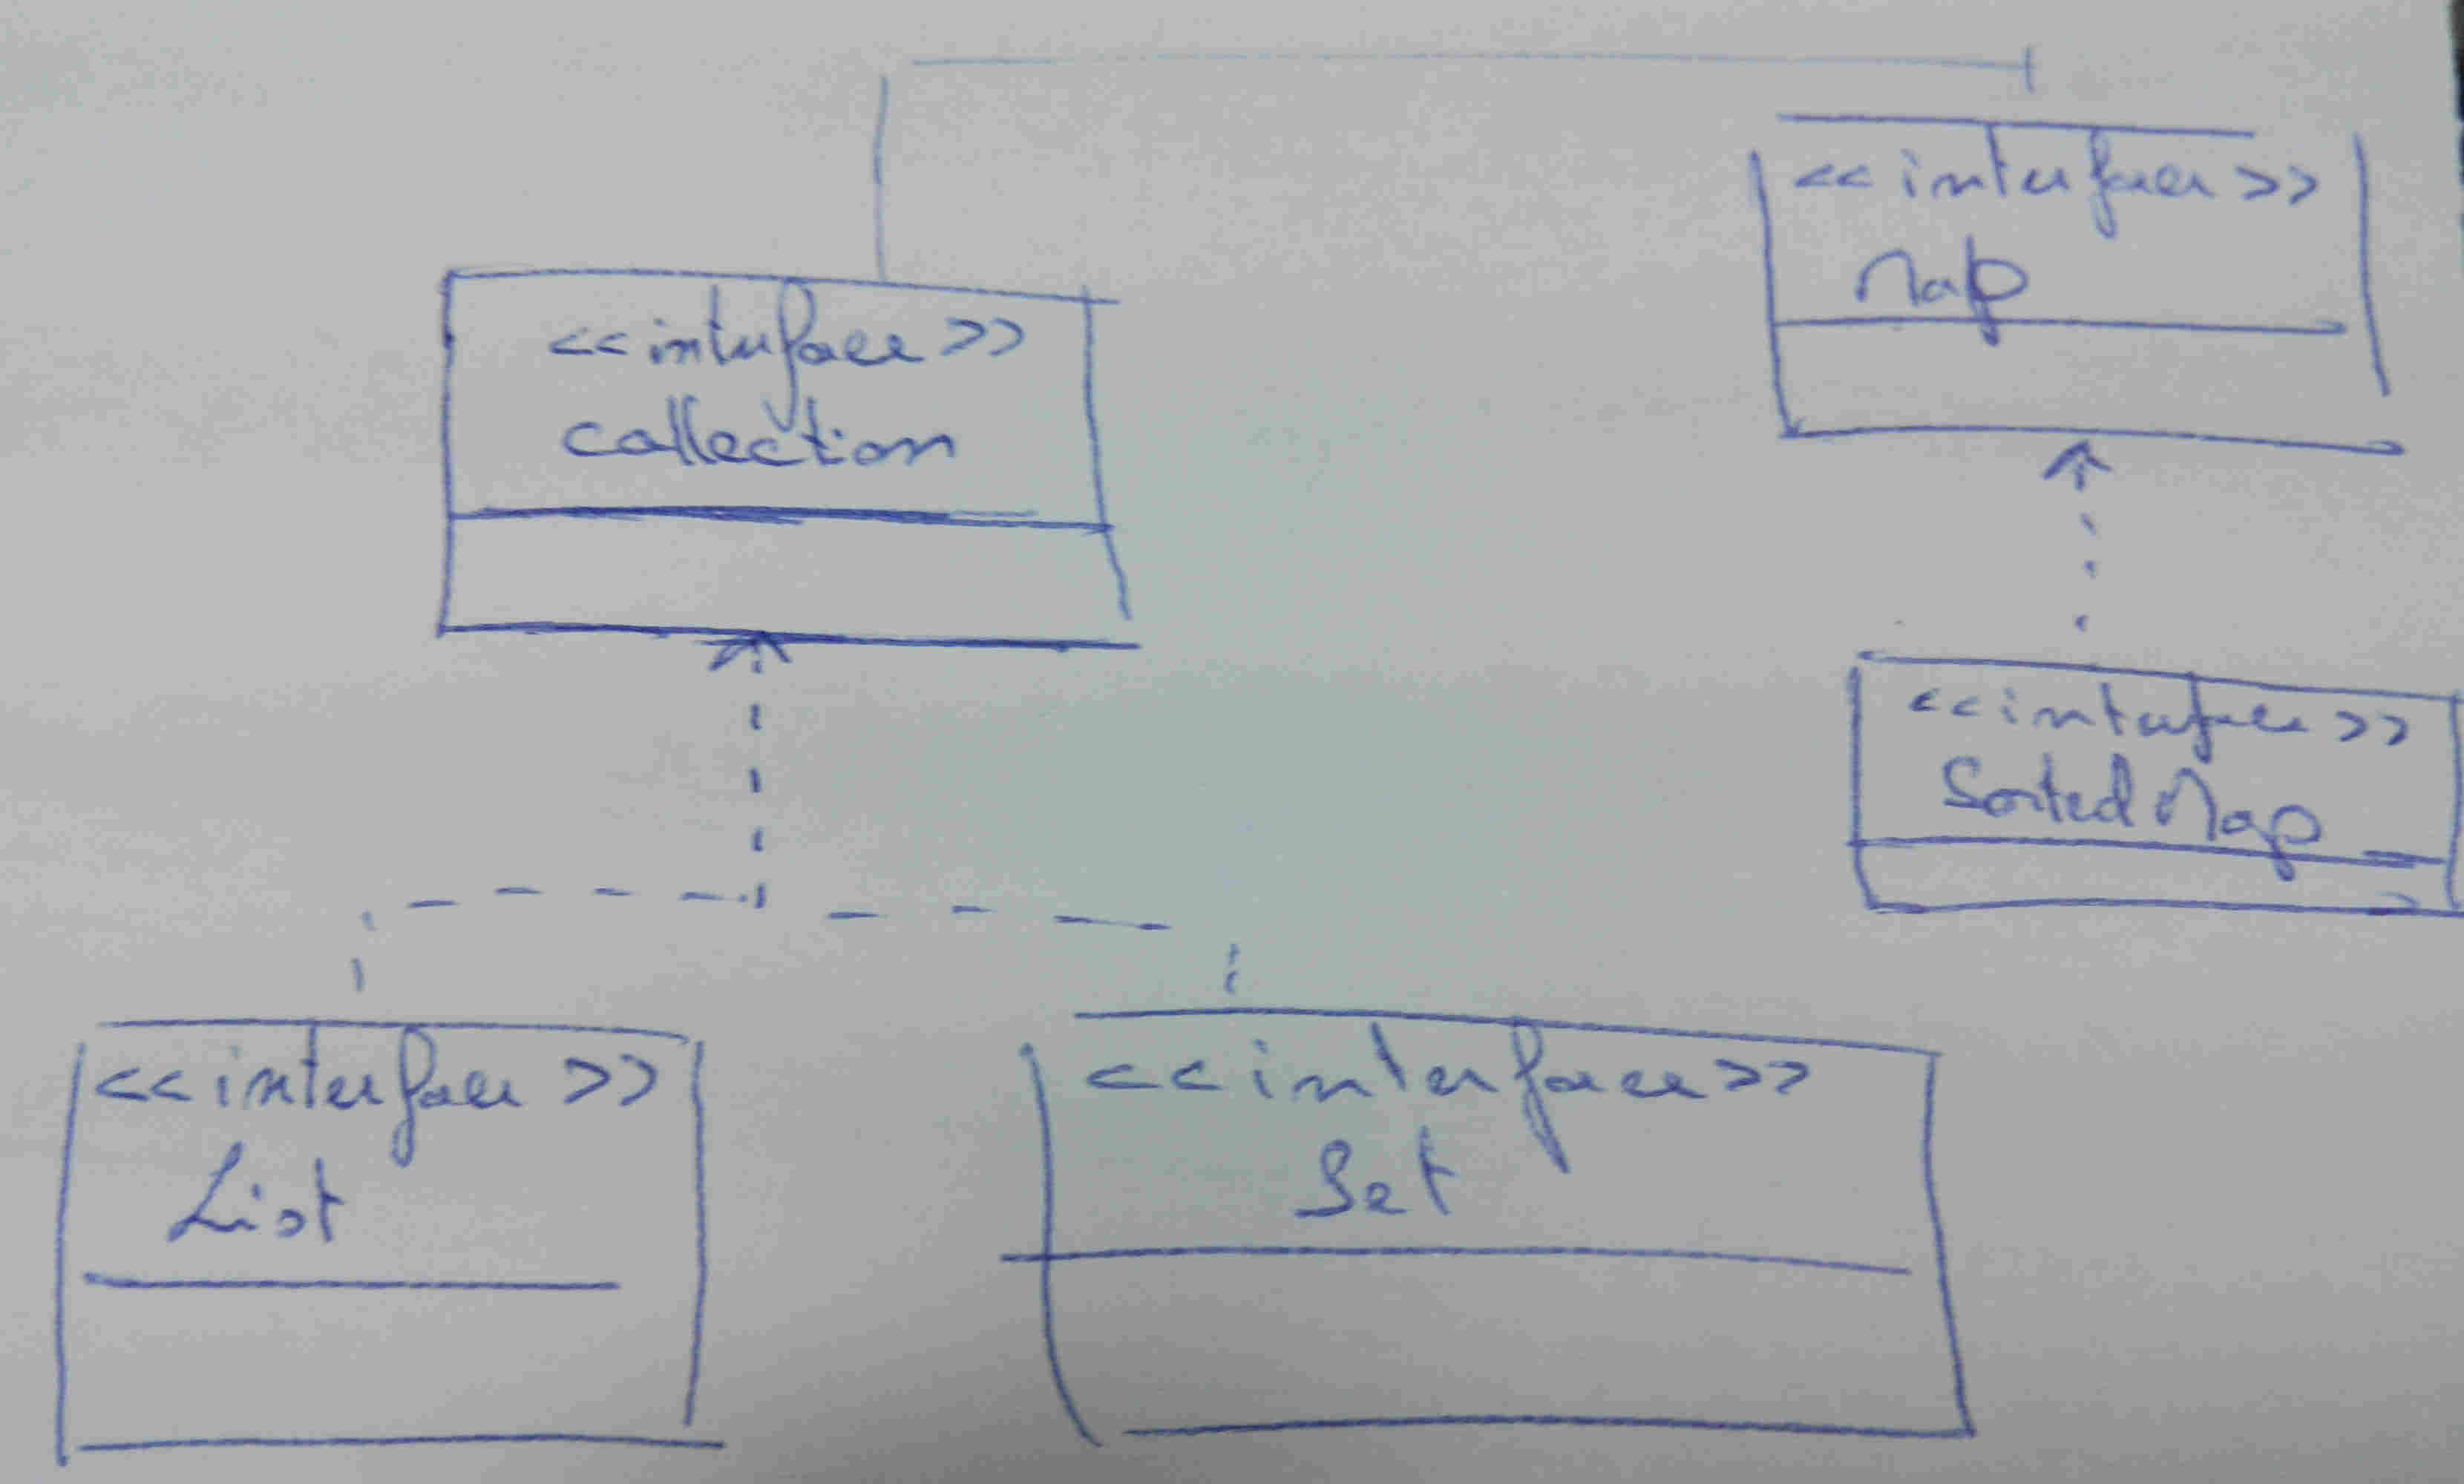
\includegraphics[scale=0.1]{image.jpg}
  \end{center}
\end{figure} \\

Le parcours est séparé du conteneur pour abstraire cette notion d'itérateur. Le but est d'utiliser une seule forme d'itérateur pour tous les types de données de ce framework pour en unifier l'utilisation. Cela masque l'implémentation, qui elle est dépendante du type de collection. \\

L'itérateur est d'ailleurs fourni par le conteneur, car sa réalisation et son implémentation dépendent de celui ci. On n'itère pas sur une liste comme sur un tableau. \\

Les Collections utilisent les types paramétrés pour permettre de détecter les incohérences de types au plus tôt, c'est-à-dire à la compilation, plutôt qu'à l'exécution. Cela oblige la personne utilisant les Collections à ne pas mélanger les types dans le conteneur, par exemple de créer une Collection mélangeant des int et des String, qui ne pourront pas être comparés.

\subsection{Remaniement de la classe Autobus}
On a ici deux choix possibles : ArrayList et LinkedList. Le code de la méthode $remove$ utilisant ArrayList :
\begin{lstlisting}
public E remove(int index) 
{
        rangeCheck(index);
        modCount++;
        E oldValue = elementData(index);
        int numMoved = size - index - 1;
        if (numMoved  > 0)
            System.arraycopy(elementData, index+1, elementData, index, numMoved);
        elementData[--size] = null; // Let gc do its work
        return oldValue;
}
\end{lstlisting}
La suppression dans le tableau est faite en décalant l'élément en question à la fin du tableau, en décalant le reste du tableau vers la gauche (pour ne pas avoir de "trous" dans le tableau), et en enlevant le lien vers l'élément à supprimer. L'élément n'étant plus référencé, le Garbage Collector va faire son travail en le supprimant. Si on passe un objet en paramètre de la méthode $remove()$, c'est $fastRemove()$ qui est appelée, et qui fait le travail précédemment décrit.\\
Le code de la méthode $remove$ utilisant LinkedList :
\begin{lstlisting}
public boolean remove(Object o) {
        if (o == null) {
            for (Node< E > x = first; x != null; x = x.next) {
                if (x.item == null) {
                    unlink(x);
                    return true;
                }
            }
        } else {
            for (Node< E > x = first; x != null; x = x.next) {
                if (o.equals(x.item)) {
                    unlink(x);
                    return true;
                }
            }
        }
        return false;
}

E unlink(Node<E> x)
{
        // assert x != null;
        final E element = x.item;
        final Node< E > next = x.next;
        final Node< E > prev = x.prev;
        if (prev == null) {
            first = next;
        } else {
            prev.next = next;
            x.prev = null;
        }
        if (next == null) {
            last = prev;
        } else {
            next.prev = prev;
            x.next = null;
        }
        x.item = null;
        size--;
        modCount++;
        return element;
}
\end{lstlisting}
Pour supprimer un élément d'une liste, on appelle la méthode unlink() (ou unlinkFirst() si c'est pour supprimer le premier). Le but ici est de rétablir les liens de la liste doublement chaînée sans le noeud de l'élément en question, (le précédent.suivant prend pour adresse le suivant du noeud de l'élément supprimé et le suivant.précédent de cet élément prend le précédent du noeud de l'élément supprimé, modulo le début et la fin de liste). Ensuite on défait le lien du noeud vers l'objet à supprimer (x.item = null). L'objet n'étant plus référencé, le Garbage Collector le supprimera.

\subsubsection{Problème}
Le binôme s'occupant de la branche factory n'a pas eu de problème lors du développement car ils ont directement choisi d'utiliser les méthodes get() et remove(), et de ne pas utiliser de copies pour faire des itérations, car copier est lourd en temps et en mémoire.\\
Cependant le deuxième binôme a en effet eu une erreur.\\
Parcourir une liste et la modifier en même temps engendre une exception de type java.util.ConcurrentModificationException. En effet, lors d'un parcours via Iterator, la Collection ne doit pas être modifiée sous peine de problème. Pour éviter ce genre de désagrément, les Iterators sont "fail-fast", c'est-à-dire qu'ils lèveront une exception ConcurrentModificationException dès qu'ils détectent la moindre modification externe.\\
En fait, il est plus judicieux d'utiliser l'Iterator "manuellement" afin d'utiliser des méthodes de modification tel que le remove(). Néanmoins, il est possible d'utiliser java.util.ListIterator qui propose des méthodes spécifique aux List.

\subsection{Solutions}
Sauf cas bien spécifique l'accès direct via index est à déconseiller au profit des Iterators. Avec une LinkedList de taille assez conséquente cela peut même s'avérer désastreux en terme de performance !\\
Une autre solution envisageable serait d'utiliser la librairie ListIterator qui permet de contourner certains problèmes, grâce au système de curseur, interne à cette classe, sur chacun des éléments de la liste.\\
Pour copier une Collection, on utilise la méthode $ArrayList<Passager> copy = passagers.clone()$. Comme dit précédemment, nous n'avons pas utilisé de copie pour supprimer un passager avec la méthode $remove()$, nous n'avons donc pas eu de problème.
\section{Commentaires}

\begin{itemize}
\item Pierre: Un des éléments principaux de ce TD était la gestion des exceptions. Il nous était proposé de le faire au TD7, c'est-à-dire une fois que l'ensemble du code est terminé et fonctionne. Cependant, je pense qu'il est plus simple de gérer les cas d'erreurs au moment où on traite les classes concernées, puisqu'on sait à ce moment là ce qui peut provoquer des erreurs. Il est plus difficile de s'en souvenir plusieurs semaines après avoir écrit le code de ces classes, même si on a plus de recul sur ce qui a été écrit.\\
Ensuite, utiliser des types de données tels que les Collections est une façon de ne pas réinventer la roue à chaque fois qu'on a à stocker des données, et utiliser des méthodes éprouvées par un grand nombre d'autres personnes, plutôt que des méthodes faites maison, qui peuvent provoquer des erreurs.\\

\item Victor: Ce projet nous a informé sur la propension du code java à gérer des exceptions. En effet, il est préférable que le programme ne s'arrête pas lorsque l'on a une erreur. Nous avons en pu pratiquer le fonctionnement, avec le chaînage qui lie la méthode de test avec la méthode qui lance l'exception, en gérant toutes les méthodes intermédiaires. \\
Enfin, nous avons pu nous informer sur d'autres types de données existants en Java, ce qui contribue une nouvelle fois, à limiter la taille de notre programme, et à le rendre plus cohérent. Ce sont des types que j'essaierai d'utiliser à l'avenir, dans mon projet PFA par exemple.\\

\item Aurélien : Ce TD nous a permis d'utiliser les exceptions pour gérer des erreurs qui ne peuvent pas l'être avec des tests unitaires. Personnellement en tant que coordinateur, j'ai pu apprécier le fait qu'une certaine mécanique s'était mise en place au sein de notre groupe après six autres TD, ce qui nous a permis de travailler de manière plus efficace. De plus j'ai trouvé ce TD intéressant dans le sens ou nous n'avons pas eu à écrire de nouvelle méthode (et les tests unitaires qui vont avec) directement utile au fonctionnement du code, ce qui change des derniers TD. \\

\item Lionel : L'issue de ce TD était la gestion des exceptions et l'utilisation des Collections. Le principe a été bien acquis et revisité pour ma part: l'utilité des exceptions existantes, la création de nos propres exceptions mais aussi ce qu'on fait une fois l'expression capturée. Ce qui confirme donc que la gestion d'exception est donc la dernière étape de la programmation d'un logiciel.\\

\item Reda : À travers ce TP, j'ai pu comprendre un peu plus les mécanismes d'exceptions. \\
De plus, l'utilisation de Collection de java.util m'a permis de prendre connaissance de types de données abstraits très utiles tels que les LinkedList ou les Map pour de futures réalisations en Java. Néanmoins, leur utilisation ne m'a pas parue très simple, le concept d'Iterator ne parait pas aussi évident. Par conséquent, il m'a semblé plus simple d'utiliser certaines méthodes qui utilisent les index pour des actions telles que la suppression.

\end{itemize}



\end{document}
